% !TeX spellcheck = en_US

\chapter{Introduction}

\begin{itemize}
	\item study computer science
	\item theoretical informatics
	\item automata theory
	\item value of this theory
	\item typical topics, why typical
	\item why automation
\end{itemize}

This work lays out the theory for a program solving this task. As a consequence, parameters, which are sensible as user input, will be incorporated in problem definitions.
In addition, when evaluating possible algorithms, we will take their usability in a practical use case into account.
Furthermore additional theory will be discussed, to enhance usability.

\section{Preliminaries}

We start with defining preliminary theoretical foundations.

\subsection{Deterministic Finite Automatons}

A 5-tuple $A = (Q, \Sigma, \delta, s, F)$ with $Q$ being a finite set of \emph{states}, $\Sigma$ a finite set of \emph{alphabet symbols}, $\delta \colon\ Q \times \Sigma \to Q$ a \emph{transition function}, $s \in Q$ a \emph{start state} and $F \subseteq Q$ \emph{final states} is called \emph{deterministic finite automaton} (DFA)~\cite[p. 46]{hopcroft01}. From now on $\mathcal{A}$ shall denote the set of all DFAs.

We say $\delta(q,\sigma) = p$ is a transition from $q$ to $p$ using symbol $\sigma$. We define the \emph{extended transition function} $\delta^* : Q \times \Sigma^* \to Q$ of a DFA $A = (Q, \Sigma, \delta, s, F)$ as:
\begin{itemize}
	\item $\delta^*(q,\varepsilon) = q$
	\item $\delta^*(q,w\sigma) = \delta(\delta^*(q,w),\sigma)$ for all $q \in Q$, $w \in \Sigma^*$, $\sigma \in \Sigma$
\end{itemize}
Then, the \emph{language} of that DFA is defined as $L(A) = \{\ w\ |\ \delta^*(w) \in F\ \}$~\cite[pp. 49-50. 52]{hopcroft01}.

Given a state $q \in Q$. With $d^-(q)$ we denote the set of all \emph{ingoing} transitions $\delta(q', \sigma) = q$ of $q$. With $d^+(q)$ we denote the set of all \emph{outgoing} transitions $\delta(q, \sigma) = q'$ of $q$~\cite[pp. 2-3]{champarnaud05}. If a transition is of the form $\delta(q, \sigma) = q$, then we say that $q$ has a \emph{loop}.

\begin{definition}\label{ch:1:unreachable-states}
	We say a state $q$ is \emph{(un-)reachable} in a DFA $A$, iff there is (no) a word $w \in \Sigma^*$ such that $\delta^*(s, w) = q$.
\end{definition}
\noindent If all states of a DFA $A$ are reachable, then we say $A$ is \emph{accessible}~\cite[p. 2]{champarnaud05}.

A DFA is called \emph{complete} iff for all states, every symbol of the alphabet is used on an outgoing transition: $\forall q\in Q\colon \forall\sigma\in\Sigma\colon \exists p\in Q\colon \delta(q,\sigma) = p$. Note, that every incomplete DFA can be converted to a complete one by adding a so called \emph{dead state}~\cite[p. 67]{hopcroft01}. The resulting automaton has the same language.

\begin{figure}
	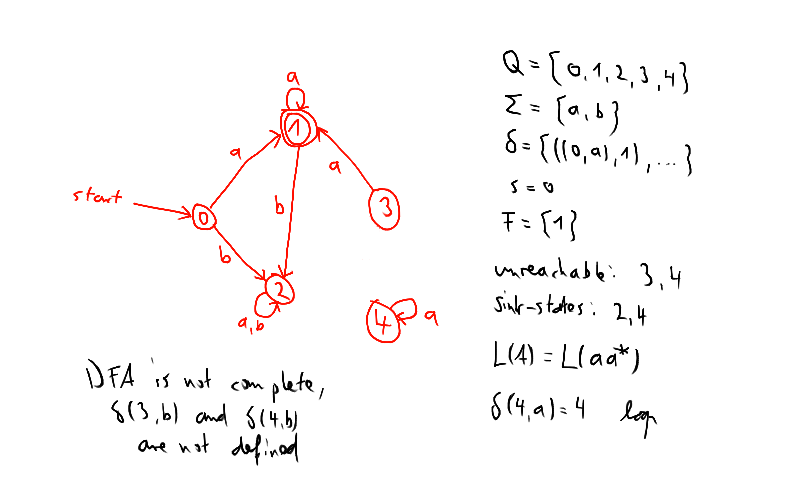
\includegraphics[width=\linewidth]{images/dfa.png}
	\caption{An example DFA and its properties.}
	\label{fig:dfa}
\end{figure}

\subsection{Minimal DFAs}

This section closely follows~\cite[pp. 42-45]{schoening01}. We call a DFA $A$ \emph{minimal}, if there exists no other automaton with the same language using less states. With $\mathcal{A}_{min}$ we shall denote the set of all minimal DFAs.

The \emph{Nerode-relation} $\equiv_L\ \subseteq\ \Sigma^* \times \Sigma^*$ of a language $L$ with alphabet $\Sigma$ is defined as follows:
\begin{displaymath}
	x \equiv_L y\ \Leftrightarrow_{def}\ \forall z\in\Sigma^*\colon (xz\in L \Leftrightarrow yz\in L)
\end{displaymath}
The Nerode-relation of a DFA $A$ is the the Nerode-relation of its language: $\equiv_{L(A)}$. If the context makes it clear, than we will shorten the notation of a equivalence class $[x]_{\equiv_L}$ with $[x]$.

The \emph{equivalence class automaton} $A_L = (Q_L, \Sigma_L, \delta_L, s_L, F_L)$ to a regular language $L$ with alphabet $\Sigma$ is defined as follows:
\begin{itemize}
	\item $Q_L = \{\ [x]\ |\ x \in \Sigma^*\ \}$
	\item $\Sigma_L = \Sigma$
	\item $\delta_L([x], \sigma) = [x\sigma],\ \forall x\in\Sigma^*,\ \forall\sigma\in\Sigma$
	\item $s = [\varepsilon]$
	\item $F = \{\ [x]\ |\ x \in L\ \}$
\end{itemize}
\begin{theorem}
	Given a language $L$, then the equivalence class automaton $A_L$ is minimal.
\end{theorem}

\subsection{Practical Isomorphy of DFAs}

Given two DFAs $A_1 = (Q_1, \Sigma_1, \delta_1, s_1, F_1)$ and $A_2 = (Q_2, \Sigma_2, \delta_2, s_2, F_2)$. We say $A_1$ and $A_2$ are \emph{practical isomorph}, iff:
\begin{itemize}
	\item $|Q_1| = |Q_2|$, $|\Sigma_1| = |\Sigma_2|$ and
	\item there exists a bijection $\phi\colon \Sigma_1 \to \Sigma_2$ such that:
	\item there exists a bijection $\pi\colon Q_1 \to Q_2$ such that:
	
	$\pi(s_1) = s_2$
	
	$\forall q\in Q_1\colon (q\in F_1 \Longleftrightarrow \pi(q)\in F_2)$
	
	$\forall q\in Q_1\colon \forall\sigma\in\Sigma_1\colon \pi(\delta_1(q,\sigma))=\delta_2(\pi(q),\phi(\sigma)))$
\end{itemize}
Note that practical isomorphy between two DFAs $A_1, A_2$ does not imply $L(A_1) = L(A_2)$. This would be given, if $\Sigma_1 = \Sigma_2$ were the case (see~\cite[p. 45]{schoening01}). However the language of such DFAs is equivalent except for an exchange of alphabet symbols:
\[
	\{\ \phi(\sigma_0)\ldots\phi(\sigma_n)\ |\ \sigma_0\ldots\sigma_n\in L(A_1)\ \} = L(A_2)
\]
%\begin{theorem} \textnormal{\cite[p. 45]{schoening01}} 
%	Every minimal DFA is unique except for isomorphy.
%\end{theorem}
%So it
%\begin{corollary}\label{ch:1:cor:all-min-dfa-ism}
%	Every minimal DFA $A$ is isomorph to its corresponding equivalence class automaton $A_{L(A)}$.
%	\gregor{All min. DFAs are ism. to each other, including A\_L}
%\end{corollary}
\gregor{Write down isomorphism test. Maybe discuss faster methods here? Look for faster methods in general?}

\subsection{Equivalent and distinguishable state pairs}

\begin{definition}[Equivalent and Distinguishable State Pairs]\cite[p. 154]{hopcroft01}
	A state pair $q_0, q_1 \in Q$ of a DFA $A = (Q, \Sigma, \delta, s, F)$ is called \emph{equivalent}, iff $\sim_A(q_0, q_1)$ is true, whereas
	\begin{displaymath}
	q_0\ \sim_A\ q_1\ \Leftrightarrow_{def}\ \forall z \in \Sigma^* \colon\ (\delta^*(q_0, z) \in F \Leftrightarrow \delta^*(q_1, z) \in F)
	\end{displaymath}
	If $(q_0, q_1) \notin \sim_A$, then $q_0$ and $q_1$ are called a \emph{distinguishable} state pair.
\end{definition}
\noindent Note that the relation $\sim_A$ is indeed an equivalence relation.

\begin{itemize}
	\item equivalent state pairs
	\item equivalent states
	\item distinguishable state pairs
	\item distinguishable states
\end{itemize}

\subsection{The minimization algorithm}

This minimization algorithm \MinAlg\ works in four major steps, removing essentially states in such a way, that no unreachable states and no equivalent state pairs are left.
\begin{enumerate}
	\item Compute all unreachable states via breadth-first search for example.
	
	\vspace{0.2cm}
	\begin{algorithmic}[1]
		\Function{\CompUnr}{$A$}
			\State $U \gets Q \setminus \{s\}$	\Comment{undiscovered states}
			\State $O \gets \{s\}$				\Comment{observed states}
			\State $D \gets \{\}$				\Comment{discovered states}
			\While {$|O| > 0$}
				\State $N \gets \{\ p\ | \ \exists q \in O\ \sigma \in \Sigma \colon\ \delta(q, \sigma) = p\ \land\ p \notin O \cup D\ \}$
				\State $U \gets U \setminus N$
				\State $D \gets D \cup O$
				\State $O \gets N$
			\EndWhile
			\State \Return $U$
		\EndFunction
	\end{algorithmic}

	\item Remove all unreachable states and their transitions.
	
	\vspace{0.2cm}
	\begin{algorithmic}[1]
		\Function{\RemUnr}{$A, U$}
			\For {$q$ \textbf{in} $U$}
				\If {$q \in F$}
					\State $F \gets F \ \{q\}$
				\EndIf
				\State $\delta \gets \delta \setminus \{\ ((q_1, \sigma), q_2) \in \delta\ |\ q_1 = q \lor q_2 = q\ \}$
			\EndFor
			\State \Return $A$
		\EndFunction
	\end{algorithmic}

	\item Compute all distinguishable state pairs ($\neg \sim_A(p, q)$).
	
	\vspace{0.2cm}
	\begin{algorithmic}[1]
		\Function{\CompDist}{$A$} \label{ch:1:minmark}
		\State $M \gets \{ (p,q), (q,p)\ |\ p \in F, q \notin F \}$
		\Do
			\State $M' \gets \{ (p,q)\ |\ (p,q) \notin M \land \exists \sigma \in \Sigma \colon (\delta(p,\sigma), \delta(q,\sigma)) \in M \}$
			\State $M \gets M \cup M'$
		\doWhile {$M' \neq \emptyset$}
		\State \Return $M$
		\EndFunction
	\end{algorithmic}
	Note that \CompDist\ requires its input automaton to be complete. \gregor{Why?}

	\item Merge all equivalent state pairs, which are exactly those, that are not in $\neg \sim_A$.
	
	\vspace{0.2cm}
	\begin{algorithmic}[1] \label{ch:1:minmerge}
		\Function{\RemEq}{$A, \neg \sim_A$}
			\State $\sim_A \gets Q^2 \setminus \neg \sim_A$
			\While {$(p,q) \in \sim_A$}
				\State $\sim_A \gets \sim_A \setminus \{ (p,q) \}$
				\If {$p = q$}
					\State \textbf{continue}
				\EndIf
				\State
				\State $Q \gets Q \setminus \{q\}$
				\If {$q \in F$}
					\State $F \gets F \setminus \{q\}$
				\EndIf
				\For {$((q_0, \sigma),q_1)$ \textbf{in} $\delta$}
					\If {$q_0 = q$}
						\State $q_0 \gets p$
					\EndIf
					\If {$q_1 = q$}
						\State $q_1 \gets p$
					\EndIf
				\EndFor
				\State
				\For {$(q_0,q_1)$ \textbf{in} $\sim_A$}
					\If {$q_0 = q$}
						\State $q_0 \gets p$
					\EndIf
					\If {$q_1 = q$}
						\State $q_1 \gets p$
					\EndIf
				\EndFor
				%\State exchange all occurrences of $q$ in $A$ and $\sim_A$ by $p$
			\EndWhile
			\State \Return $A$
		\EndFunction
	\end{algorithmic}
	Note that \RemEq\ preserves completeness, since it does only remove transitions from those state, that are removed anyway from the automaton.
	\gregor{\RemEq\ constructs possibly nondet. DFAs on its way. Write it more explicit. Probably someone has?}
\end{enumerate}
\begin{theorem}
	The minimization algorithm computes a minimal DFA to its input DFA.
\end{theorem}
\noindent The definition of this DFA minimization algorithm is inspired by Schöning~\cite[p. 46]{schoening01}.

\paragraph*{$m$-\CompDist.}

When looking at \CompDist, one notes, that it computes distinct subsets of $Q \times Q$ on the way. Indeed, one could write the algorithm in such a way, that these subsets are explicitly computed in form of a function $m\colon\mathbb{N}\to\mathcal{P}(Q\times Q)$:
\vspace{0.2cm}
\begin{algorithmic}[1] \label{ch:1:m-minmark}
	\Function{$m$-\CompDist}{$A$}
	\State $i \gets 0$
	\State $m(0) \gets \{ (p,q), (q,p)\ |\ p \in F, q \notin F \}$
	\Do
		\State $i \gets i + 1$
		\State $m(i) \gets \{ (p,q)\ |\ (p,q) \notin \bigcup{m(\cdot)} \land \exists \sigma \in \Sigma \colon (\delta(p,\sigma), \delta(q,\sigma)) \in m(i-1) \}$
	\doWhile {$m(i) \neq \emptyset$}
	\State \Return $\bigcup{m(\cdot)}$
	\EndFunction
\end{algorithmic}
\vspace{0.2cm}
Using this redefinition, we can easier refer to the state pairs marked in a certain iteration. We will use both variants in exchange.

We will denote the number of iterations done by \CompDist\ on an DFA $A$ as $\mmD(A)$. Note that $\mmD(A) = \max n \in \mathbb{N}\ |\ m(n) \neq \emptyset$. \gregor{Does that note maybe fit very well to the proof of lemma~\ref{ch:3:semantics-of-D(A)}?}

\subsection{Essential and redundant states}

When looking at \CompDist\ and \RemEq\ one furthermore notes, that they essentially
\begin{enumerate}
	\item compute the equivalence classes of $\sim_A$ (by exploring for each state pair whether its equivalent)
	
	$eq\_classes(\sim_A) = \{ [q]_{\sim_A} | q \in Q \} = \{C_0,\ldots,C_n\}$
	\item choose one state $e_i$ of each equivalence class $C_i$ and merge all other states towards it (\RemEq\ never creates new states, but transfers transitions)
\end{enumerate}
These dedicated states $e_0, \ldots, e_n$ then correspond exactly to the states of the equivalence automaton - each state represents one equivalence class, and every equivalence class is represented by one state.

Since \MinAlg\ can be applied to any DFA, we can be sure that there exist states $e_0, \ldots, e_n$ in every automaton $A$, which would remain as set of states for the automaton \MinAlg($A$). We shall name these states \emph{essential} states. All states that will not be part of the by \MinAlg\ minimized DFA will be called \emph{redundant} states.

\gregor{Example: In~\ref{fig:dfa_ex_task} and~\ref{fig:dfa_ex_sol} the state pairs $(A,D), (C,E)$ are equivalent and all others distinguishable. The states $A, G, C, B$ are essential, for they show up in the minimized automaton. The states $D, E$ are therefore redundant.}

As a consequence saying that \RemEq\ \emph{merges equivalent state pairs} is equivalent to saying it \emph{removes redundant states}.

\section{Requirements analysis}

Now that we have introduced all necessary basic definitions, we shall do a short analysis of an example DFA minimization task and its sample solution, as it could have been given to students in an introductory course to automata theory.

\subsection{Example of a DFA minimization task for students}

\begin{itemize}
	\item search for typical test in text standard work books
\end{itemize}

\begin{figure}
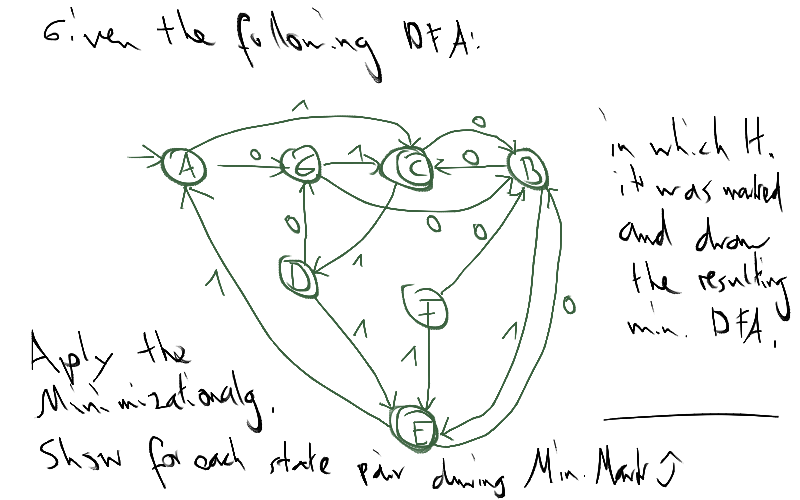
\includegraphics[width=\linewidth]{images/dfa_ex_task.png}
\caption{An example DFA minimization task.}
\label{fig:dfa_ex_task}
\end{figure}

\begin{figure}
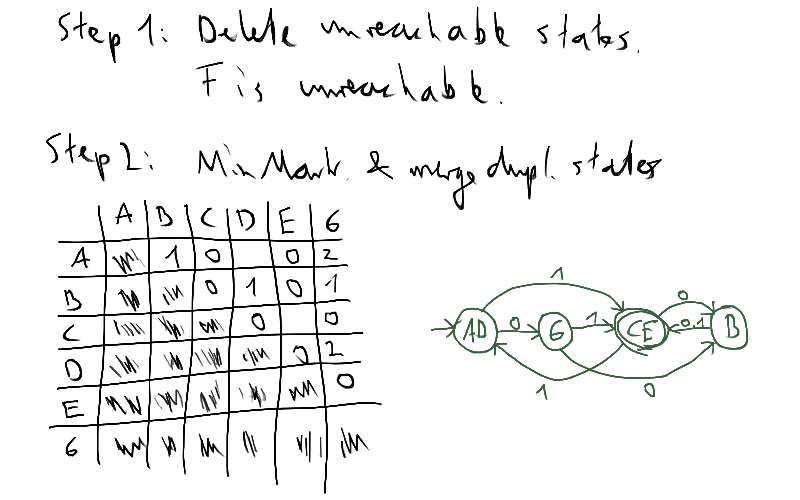
\includegraphics[width=\linewidth]{images/dfa_ex_sol.png}
\caption{Solution to the DFA minimization task in fig.~\ref{fig:dfa_ex_task}.}
\label{fig:dfa_ex_sol}
\end{figure}

\noindent Figures and~\ref{fig:dfa_ex_sol} show such a task and solution. In a DFA minimization task (fig.~\ref{fig:dfa_ex_task}) students are confronted with a \emph{task DFA} $A_{task}$, that is to be minimized by eliminating unreachable states (thus gaining the \emph{intermediate DFA} $A_{inter}$) and merging equivalent state pairs towards a \emph{solution DFA} $A_{sol}$ using the minimization algorithm. The table $T$ displayed in the solution is nothing else but a visualization of the function $m$, whereas $T(q_0, q_1) = i \Leftrightarrow (q_0, q_1) \in m(i)$. 

There are some formal statements and requirements. Firstly, we can state that
\begin{itemize}
	\item $A_{inter} = \RemUnr(A_{task}, \CompUnr(A_{task}))$ and
	\item $A_{sol} = \RemEq(A_{inter}, \CompDist(A_{inter}))$
\end{itemize}
Therefore $A_{sol}$ has to be minimal regarding $A_{inter}$ and $A_{task}$. Secondly the languages of $A_{task}, A_{inter}$ and $A_{sol}$ must be equal. We know that \CompDist\ requires $A_{inter}$ to be complete and that \RemEq\ preserves completeness, so $A_{sol}$ is complete too. Furthermore we know that every state of $A_{reach}$ reachable since it is the output of \RemUnr.

\gregor{How to define 'already found DFA sol' as requirement}

\subsection{Difficulty adjustment possibilities}

Concerning the execution of \MinAlg\ we find that its difficulty can be classified through various classification numbers.

\paragraph*{\CompDist-depth ($\mmD(A_{task})$).}

Consider the computation of the sets $m(i)$ in \CompDist. Determining $m(0)$ is quite straightforward, because it consists simply of tests whether two states are in $F \times Q \setminus F$ (see~\ref{ch:1:m-minmark}, line 3). Determining $m(1)$ is less easy: The rule for determining all $m(i), i > 0$ is different to that for $m(0)$ and more complicated (see~\ref{ch:1:m-minmark}, line 6). Determining $m(2)$ requires the same rule. It shows nonetheless a students understanding of the terminating behavior of \CompDist: It does not stop after computing $m(1)$, but only when no more distinguishable state pairs were found. Concerning the sets $m(i), i > 2$ however no additional understanding can be shown.

It would therefore be sensible if $\mmD(A_{task})$ could be adjusted for example by parameters $m_{min}, m_{max}$ which give lower and upper bounds for that value.

\paragraph*{Number of unreachable and redundant states.}

The task DFA contains $u$ unreachable states and $r$ redundant states. It is sensible to have $u > 1, r > 1$, such that \RemUnr\ and \RemEq\ will not be skipped. A exercise instructor will find it useful, to control exactly how big $u$ and $r$ are: The higher $u, r$, the more states have to be eliminated and merged.

\paragraph*{Number of states alltogether ($|Q_{task}|$).}

The more states $A_{task}$ has, the higher is the number of state pairs, which have to be checked. Thus a possiblity to adjust also the number of reachable and redundant states, denoted $q$, would be useful. Note that $|Q_{task}| = |Q_{inter}| + d = |Q_{sol}| + u + d$ so $q = |Q_{sol}|$.

\paragraph*{Alphabet size ($|\Sigma|$).}

The more symbols the alphabet of $A_{task}, A_{inter}$ and $A_{sol}$ has, the more transitions have to be followed when checking whether $(\delta(q,\sigma),\delta(p,\sigma))\in m(i-1)$ is true for each state pair $p,q$.

\paragraph*{Completeness of $A_{task}$.}

Even though \CompUnr\ and \RemUnr\ do not require their input DFA $A_{task}$ to be complete, it is sensible to build it that way. The implications of the completeness-property are - in comparison to the other concepts involved here - rather subtle. This is especially due to its purely representational nature, a DFA has the same language and $\mmD$-value, whether it is represented in its complete form or not. Nonetheless we shall introduce a parameter $c$, that determines if there exist unreachable states, that make $A_{task}$ incomplete. Thus an exercise lecturer could showcase this matter on a DFA and generate according exercises.

\paragraph*{Planar drawing of $A_{task}$.}

A graph $G$ is \emph{planar} if it can be represented by a drawing in the plane such that its edges do not cross. Such a drawing is then called \emph{planar drawing} of $G$. A visual aid for students would be given, if the task DFA were planar and presented as a planar drawing. In this work libraries will be used to allow the option of planarity, but neither ensuring planarity nor planar drawing will be investigated further theoretically.

\paragraph*{Maximum degree of any state in $A_{task}$.}

The \emph{degree} $deg(q)$ of a state $q \in Q$ in a DFA $A$ is defined as $deg(q) = |d^-(q)| + |d^+(q)|$, so the total number of transitions in which $q$ participates. By capping the maximum degree for all states, the graphical representation of the DFA would be more clear. In this work the inclusion of a maximum degree parameter is omitted.

%Note that $deg(q) \geq |\Sigma|$ for any complete DFA, since states of complete DFAs have to use all alphabet symbols on outgoing transitions.

\subsection{Summary}

\label{ch:1:determined-requirements}
Accepted general criteria:
\begin{itemize}
	\item[->] $L(A_{sol}) = L(A_{inter}) = L(A_{task})$
	\item[->] $\mmD(A_{sol}) = \mmD(A_{inter}) = \mmD(A_{task})$
\end{itemize}
Accepted solution DFA criteria:
\begin{itemize}
	\item[->] has to be minimal, complete
	\item[->] number of states
	\item[->] number of \CompDist\ iterations ($\mmD(A_{sol})$)
	\item[->] alphabet size
	\item[->] number of accepting states
	\item[->] planarity
	\item[->] $A_{sol}$ is new
	
	\begin{definition}[New DFAs] \label{ch:1:new-dfa}
		A DFA $A_{sol}$ is \emph{new} if it is not practically isomorph to any previously generated solution DFA.
	\end{definition}
\end{itemize}
Accepted intermediate DFA criteria:
\begin{itemize}
	\item[->] has to be complete
	\item[->] number of unreachable states
	\item[->] planarity (can be checked in $O(|Q_{task}|)$)
\end{itemize}
Accepted task DFA criteria:
\begin{itemize}
	\item[->] number of redundant states
	\item[->] planarity
	\item[->] completeness
\end{itemize}

\section{Approach and general algorithm}

In this work we will first build the solution DFA (step 1), and - based on that - the task DFA by adding unreachable and redundant states(step 2). Both steps will fulfill all criteria chosen above and are covered in depth in chapter~\ref{ch:2} respectively chapter~\ref{ch:3}.

It follows that $\mmD$ and $L$ of both DFAs will be set when building $A_{sol}$. As a consequence we need to ensure that adding redundant and unreachable state does neither change $\mmD(A_{task})$ nor $L(A_{task})$ in comparison to $A_{sol}$. We will do this during the discussion of step 2.

Here follow problem definitions for the two steps, which specify all needed informations. \gregor{Hidden formulation here} %The first problem is lain out in a way, such that it does

\begin{definition}[BuildNewMinimalDFA] \label{ch:1:def:BuildNewMinimalDFA} $ $
	\begin{description}
		
		\item[Given:] $ $
		
		$q, a, f, m_{min}, m_{max} \in \mathbb{N},$
		
		$p \in \{0,1\}$
		\item[Request:] $ $
		
		Let $A_{sol} = (Q, \Sigma, \delta, s, F)$ be a DFA, such that
		
		\qquad $|Q|=q$, $|\Sigma|=a$, $|F|=f$,
		
		\qquad $m_{min} \le \mmD(A_{sol}) \le m_{max}$,
		
		\qquad $A_{sol}$ is planar iff $p = 1$ and
		
		\qquad $A$ is new
		
		Return $A_{sol}$, if it exists, $\bot$ otherwise.
	\end{description}
\end{definition}

\begin{definition}[ExtendMinimalDFA] \label{ch:1:def:ExtendMinimalDFA} $ $
	\begin{description}
		
		\item[Given:] $ $
		
		$A_{sol} = (Q, \Sigma, \delta, s, F) \in \mathcal{A}_{min},$
		
		$p \in \{0,1\},$
		
		$r, u \in \mathbb{N}$
		\item[Request:] $ $
		
		A DFA $A_{task} = (Q', \Sigma', \delta', s', F')$ with reachable redundant states $q_1 \ldots q_r$ and unreachable states $p_1 \ldots p_u$, such that
		
		$Q = Q' \cup \{ q_1, \ldots q_r, p_1 \ldots p_u \}$,
		
		$\Sigma = \Sigma'$, $s = s'$,
		
		$F \subseteq F'$,
		
		$A_{task}$ is planar iff $p = 1$,
		
		$L(A_{sol}) = L(A_{task})$ and $\mmD(A_{sol}) = \mmD(A_{task})$.
	\end{description}
\end{definition}

\noindent The main algorithm will then simply be:
\vspace{0.2cm}
\begin{algorithmic}[1]
	\Function{GenerateDFAMinimizationProblem}{$q, a, f, m_{min}, m_{max}, p_1, p_2, d, u$}
	\State $A_{sol} \gets \textsc{BuildNewMinimalDFA}(q, a, f, m_{min}, m_{max}, p_1)$
	\State $A_{task} \gets \textsc{ExtendMinimalDFA}(A_{sol}, p_2, r, u)$
	\State \Return $A_{sol}, A_{task}$
	\EndFunction
\end{algorithmic}


